% Options for packages loaded elsewhere
\PassOptionsToPackage{unicode}{hyperref}
\PassOptionsToPackage{hyphens}{url}
\PassOptionsToPackage{dvipsnames,svgnames*,x11names*}{xcolor}
%
\documentclass[
]{article}
\usepackage{lmodern}
\usepackage{amssymb,amsmath}
\usepackage{ifxetex,ifluatex}
\ifnum 0\ifxetex 1\fi\ifluatex 1\fi=0 % if pdftex
  \usepackage[T1]{fontenc}
  \usepackage[utf8]{inputenc}
  \usepackage{textcomp} % provide euro and other symbols
\else % if luatex or xetex
  \usepackage{unicode-math}
  \defaultfontfeatures{Scale=MatchLowercase}
  \defaultfontfeatures[\rmfamily]{Ligatures=TeX,Scale=1}
\fi
% Use upquote if available, for straight quotes in verbatim environments
\IfFileExists{upquote.sty}{\usepackage{upquote}}{}
\IfFileExists{microtype.sty}{% use microtype if available
  \usepackage[]{microtype}
  \UseMicrotypeSet[protrusion]{basicmath} % disable protrusion for tt fonts
}{}
\makeatletter
\@ifundefined{KOMAClassName}{% if non-KOMA class
  \IfFileExists{parskip.sty}{%
    \usepackage{parskip}
  }{% else
    \setlength{\parindent}{0pt}
    \setlength{\parskip}{6pt plus 2pt minus 1pt}}
}{% if KOMA class
  \KOMAoptions{parskip=half}}
\makeatother
\usepackage{xcolor}
\IfFileExists{xurl.sty}{\usepackage{xurl}}{} % add URL line breaks if available
\IfFileExists{bookmark.sty}{\usepackage{bookmark}}{\usepackage{hyperref}}
\hypersetup{
  pdftitle={Data Exploration: Cooperation},
  pdfauthor={Your name here},
  colorlinks=true,
  linkcolor=Maroon,
  filecolor=Maroon,
  citecolor=Blue,
  urlcolor=blue,
  pdfcreator={LaTeX via pandoc}}
\urlstyle{same} % disable monospaced font for URLs
\usepackage[margin=1in]{geometry}
\usepackage{graphicx,grffile}
\makeatletter
\def\maxwidth{\ifdim\Gin@nat@width>\linewidth\linewidth\else\Gin@nat@width\fi}
\def\maxheight{\ifdim\Gin@nat@height>\textheight\textheight\else\Gin@nat@height\fi}
\makeatother
% Scale images if necessary, so that they will not overflow the page
% margins by default, and it is still possible to overwrite the defaults
% using explicit options in \includegraphics[width, height, ...]{}
\setkeys{Gin}{width=\maxwidth,height=\maxheight,keepaspectratio}
% Set default figure placement to htbp
\makeatletter
\def\fps@figure{htbp}
\makeatother
\setlength{\emergencystretch}{3em} % prevent overfull lines
\providecommand{\tightlist}{%
  \setlength{\itemsep}{0pt}\setlength{\parskip}{0pt}}
\setcounter{secnumdepth}{-\maxdimen} % remove section numbering

\title{Data Exploration: Cooperation}
\author{Your name here}
\date{September 16, 2021}

\begin{document}
\maketitle

To begin this assignment, \textbf{make sure you have downloaded all the
materials in this week's folder on Canvas}. Before you begin, make sure
you have the files \texttt{data\_assignment\_sept16.Rmd} and
\texttt{data\_assignment\_sept16.pdf} as well as the folders
\texttt{axelRod-master} and \texttt{rmd\_photos} in the same folder on
your computer. You will be using a Shiny app, developed by
\href{https://github.com/swarm-lab/axelRod/tree/master/R}{Simon Garnier}
and edited slightly by the TF team, that will only work if those things
are all in the same place.

Next, \textbf{you must set your working directory to the source file
location}. To do so, select `Session' from the menu bar at the top of
your screen, hover over `Set Working Directory', then select `To Source
File Location'.

When knitting your RMarkdown file to a PDF, make sure to say ``No'' when
it asks you if you would like to ``Render and view this document using
Shiny instead.''

If you have trouble getting the Shiny app to work (or with anything
else), please come to the teaching team. We are happy to help!

\hypertarget{the-evolution-of-cooperation}{%
\section{The Evolution of
Cooperation}\label{the-evolution-of-cooperation}}

Axelrod's \textit{Evolution of Cooperation} uses the construct of the
Prisoner's Dilemma to illustrate how cooperation can emerge despite
incentives not to. In the Prisoner's Dilemma game, players must choose
whether to cooperate or defect. The payoffs for doing one or the other
depend on what the other player does, but no matter if the other player
cooperates or defects, it is always strictly better for players to
defect.

This can be seen in the table below, which replicates the game Axelrod
uses throughout his book. If player 2 cooperates, it's better for player
1 to defect, since then player 1 would receive 5 points instead of 3. If
player 2 defects, player 1 definitely wants to defect and receive 1
point rather than 0. So no matter what each player expects the other to
do, they will both choose to defect, yielding 1 point to each player.

\begin{center}
\begin{tabular}{ | c | c | c | } 
\hline
P1 $\downarrow$; P2 $\rightarrow$ & C & D \\ 
\hline
C & R = 3, R = 3 & S = 0, T = 5 \\ 
\hline
D & T = 5, S = 0 & P = 1, P = 1 \\ 
\hline
\end{tabular}
\end{center}

But ideally, in the long run (in a repeated game) players would like to
cooperate and receive 3 points on each round. Axelrod explains how
strategies of cooperation can evolve even in circumstances where players
are antagonists (like Allied and Axis soldiers in the trenches of World
War I) or when the players are not capable of foresight (as is the case
for cooperation in biological systems).

\hypertarget{the-prisoners-dilemma-simulator}{%
\section{The Prisoner's Dilemma
Simulator}\label{the-prisoners-dilemma-simulator}}

For this week's Data Exploration assignment, you will be working with a
Shiny app that simulates prisoner's dilemma games. To use it, simply run
the code chunk above labeled `setup', then run the following code
(\texttt{shiny\_tournament()}). Doing so will open the app in a separate
window.

P.S., the ``Instructions'' tab in the app is broken. Don't worry if it
doesn't display anything for you. Refer to this document for
instructions.

P.P.S., when you close the app window, there may be some warnings or
errors (like ``no loop for break/next, jumping to top level''). You can
just ignore them.

\hypertarget{setup}{%
\subsection{Setup}\label{setup}}

Now we're going to do a round-robin style tournament between strategies
of your choosing, similar to the ones Axelrod conducted. All students
must complete this part, as the subsequent questions are based on the
tournament you conduct here.

\textbf{First}, choose at least 6 strategies from the menu that look
interesting to you. Your task is to play each one against all the other
opponents and record the results in the excel file available in the
Google Drive called \texttt{prisoners\_dilemma\_data.xlsx}.

\textbf{Second}, once you have chosen your strategies, type all the
pairwise combinations of those strategies into the columns
\texttt{player1} and \texttt{player2}. Make sure you type the strategies
exactly as they appear in the application, including the case of the
letters! Your spreadsheet should look this like after you have done so
(but with the strategies you choose):

\begin{figure}
\centering
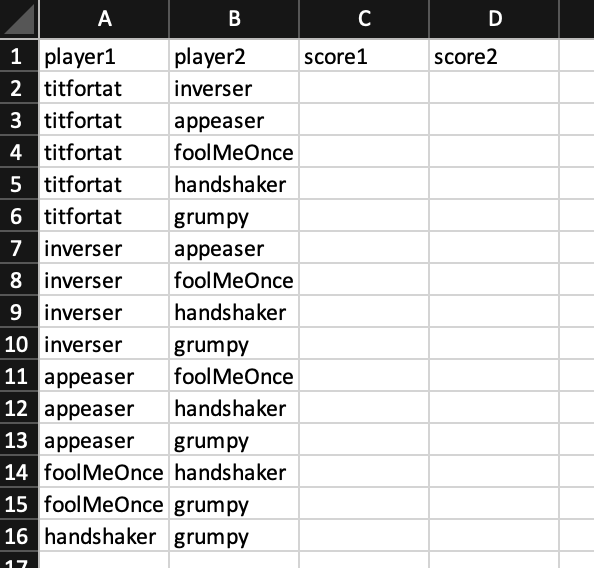
\includegraphics{./rmd_photos/step2.png}
\caption{This is what your table should look like after step 2.}
\end{figure}

Note that there are 15 ways to combine 6 elements into
pairs\footnote{In math terms, this results from the fact that ${6 \choose 2} = 15$},
so if you don't have 15 pairs, check your work. Also note that the more
strategies you choose, the more typing you will have to do.

\textbf{Third}, set the app so that ``Tournament Type'' = ``Repeated'',
``Number of Rounds'' = 100, and ``Number of Replications'' = 100. Just
as in Axelrod's simulation, we are playing repeated games (this is
determined by the ``Number of Rounds''). The ``Number of Replications''
changes how many times the computer plays each repeated game. So in the
example above, the computer will repeat the 100-round game of titfortat
vs.~inverser 100 times over and take the average outcome of each of
those replications. This is useful because some of the strategies rely
on probability (e.g.~play ``Defect'' with probability .5) and so the
outcome will be different each time. We average over many outcomes to
see which strategy wins on average. Once you're done, your spreadsheet
should look something like this, but with different strategies:

\begin{figure}
\centering
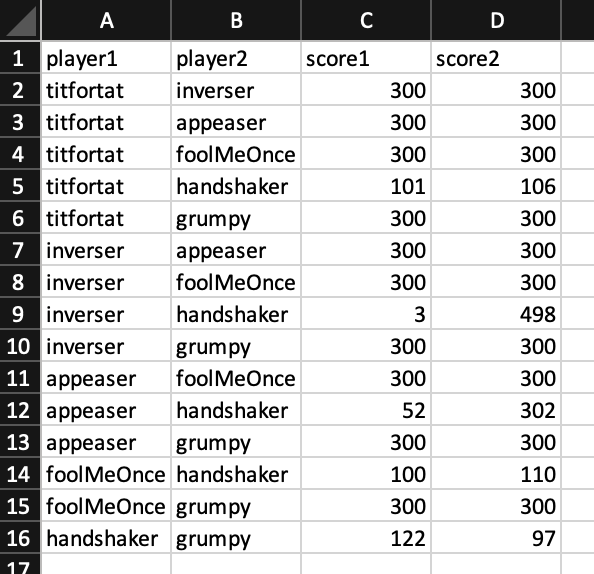
\includegraphics{./rmd_photos/step3.png}
\caption{This is what your table should look like after step 3.}
\end{figure}

Of course, don't just copy these numbers, since they're made up.

\textbf{Fourth}, save the file as a CSV. To do so, go to File
\textgreater{} Save As, then set the File Format to be
\texttt{CSV\ UTF-8\ (Comma\ delimited)\ (.csv)}. Make sure to save it
with the name \texttt{prisoners\_dilemma\_data.csv}.

Now you can finally read the data you created into R using the following
code and start answering the questions that follow.

\hypertarget{question-1}{%
\subsection{Question 1}\label{question-1}}

\textbf{How do the strategies you chose rank against each other based on
the number of wins? How do they rank based on the number of points won?
Discuss the patterns you see here as they relate to what you read from
Axelrod. Keep in mind the concepts of niceness, retaliation,
forgiveness, and clarity.}

The following code makes a data frame called \texttt{player\_data\_long}
that you can use to rank the strategies based on the number of points
won during the tournament. As a hint, you may want to try using
\texttt{group\_by()}, \texttt{summarize()}, and \texttt{arrange()} on
\texttt{player\_data\_long}.

If you want, try to figure out what each line of code does. Cleaning the
data and rearranging it like this is an important part of data science,
not just running regressions and taking means. This is why we are
leaving some of it to you, via \texttt{group\_by()} and
\texttt{summarize()}.

To rank the strategies based on the number of wins, think about making
use of the \texttt{winner} variable in the \texttt{pda\_data} data
frame.

\hypertarget{question-2}{%
\subsection{Question 2}\label{question-2}}

\textbf{Make a plot like the one below that displays how your winning
strategy (according to total points) fared against the strategies it
played against. Using \texttt{player\_data\_long} is probably easiest,
but complete this question however makes most sense to you. Comment on
what you find.}

\begin{figure}
\centering
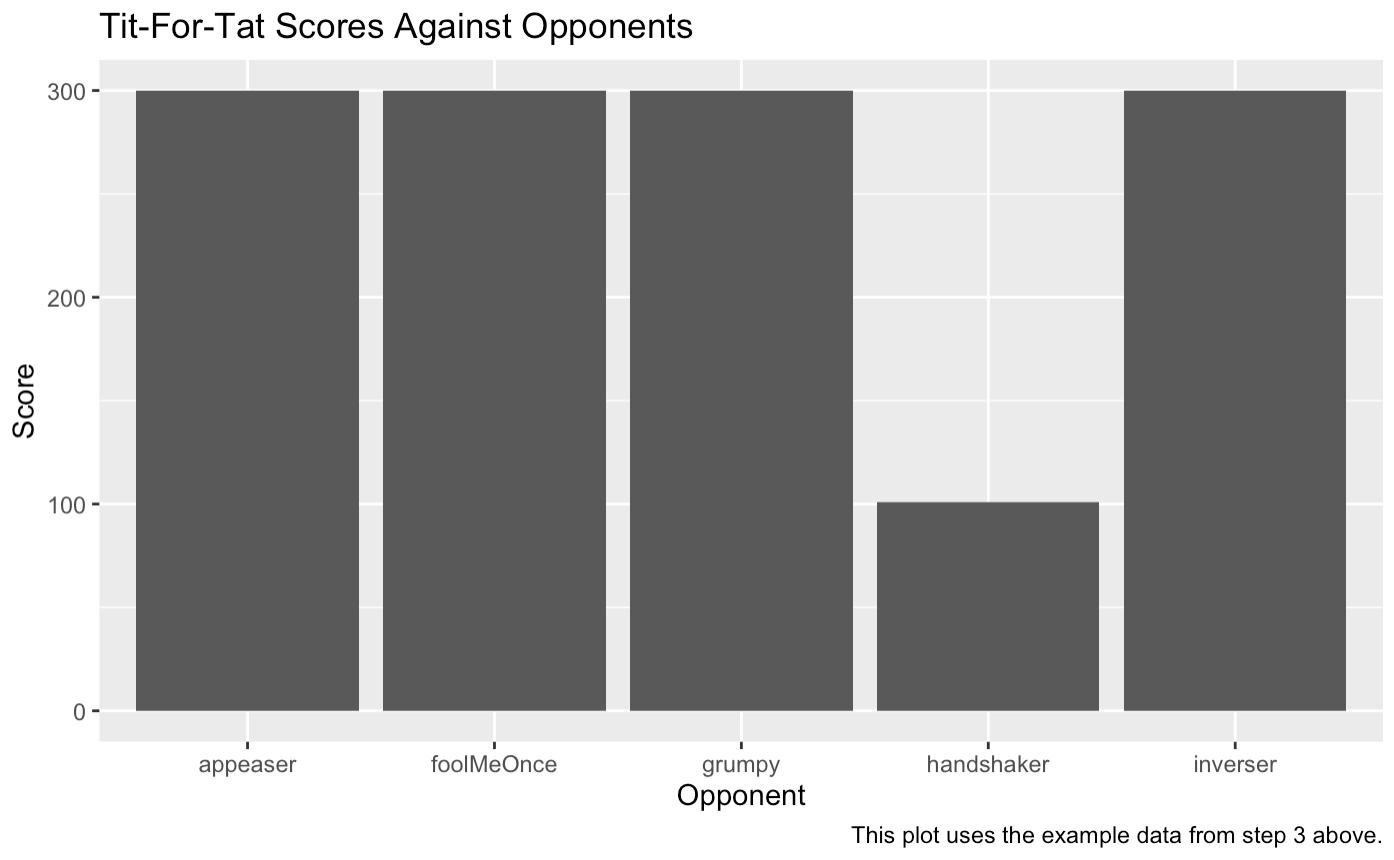
\includegraphics{./rmd_photos/question2.png}
\caption{Here is an example of a plot you might make.}
\end{figure}

\hypertarget{question-3-data-science-question}{%
\subsection{Question 3: Data Science
Question}\label{question-3-data-science-question}}

\textbf{Create a plot, similar to the one above, that displays how each
strategy fared against all the other strategies. Which strategies were
most successful against which other ones? Comment on the patterns that
you see.}

\includegraphics{data_assignment2_sept_16_2021_files/figure-latex/make_plot-1.pdf}

\hypertarget{question-4}{%
\subsection{Question 4}\label{question-4}}

\textbf{What is the main difference between the game you played here and
the tournament Axelrod implemented? How do you think this difference
might matter?}

\end{document}
